\documentclass[UTF8]{ctexart}
\usepackage{geometry}
\usepackage{listings}
\usepackage{xcolor}
\usepackage{graphicx}
\usepackage{float}
\usepackage{multirow}
\usepackage{array}
\usepackage{longtable}
\usepackage{hyperref}
\usepackage{ctex}

\geometry{a4paper,scale=0.8}
\lstset{
    numbers=left, %设置行号位置
    numberstyle=\tiny, %设置行号大小
    keywordstyle=\color{blue}, %设置关键字颜色
    commentstyle=\color[cmyk]{1,0,1,0}, %设置注释颜色
    frame=single, %设置边框格式
    escapeinside=``, %逃逸字符(1左面的键),用于显示中文
    breaklines, %自动折行
    extendedchars=false, %解决代码跨页时,章节标题,页眉等汉字不显示的问题
    xleftmargin=2em,xrightmargin=2em, aboveskip=1em, %设置边距
    tabsize=4, %设置tab空格数
    showspaces=false %不显示空格
    }
\hypersetup{
    colorlinks=true,
    linkcolor=black,
    citecolor=black
}
\title{计算机系统结构实验报告\\实验4}

\date{\today}
\begin{document}
\maketitle
\begin{abstract}
    本实验实现了简单的类MIPS处理器的几个重要部件:寄存器(Register)、数据内存(Data Memory)以及符号扩展模块(Sign Extension),其作用分别是暂时存放一些数据与运算结果、用于较大量存储数据以及对立即数进行扩展。对于存储部件(如寄存器、存储器等),其需要实现读取数据、存放数据和写入数据的功能。对于符号扩展部件,其需要根据控制信号进行无符号扩展或带符号扩展。本实验通过软件仿真的形式进行实验结果的验证。
  \end{abstract}  
\tableofcontents
\clearpage
\section{实验目的}
\begin{enumerate}
    \item 理解 CPU 的寄存器、存储器、无符号扩展、带符号扩展的原理
    \item 寄存器模块的实现
    \item 数据内存模块的实现
    \item 符号扩展模块的实现
    \item 功能仿真
\end{enumerate}
\section{原理分析}
\subsection{寄存器模块}
寄存器(Register)是中央处理器内用来暂存指令、数据和地址的存储器。寄存器的存贮容量有限,读写速度非常快。在计算机体系结构里,寄存器存储在已知时间点所作计算的中间结果,通过快速地访问数据来加速计算机程序的运行。\par
本实验中,寄存器模块总共有32个寄存器,因此需要使用5位选择信号对寄存器进行寻址。每个寄存器的长度为32位,对于处理器的一个字长,因此数据输入与输出均为32位。
\par
寄存器模块的输入与输出信号如表\ref{tab:reg-input-sig}与表\ref{tab:reg-output-sig}所示。
\begin{table}[htbp]
    \centering
    \begin{tabular}{|c|c|c|}
    \hline
    输入信号 & 长度 & 说明 \\
    \hline
    readReg1 & 5 & 读取寄存器1的编号 \\
    readReg2 & 5 & 读取寄存器2的编号 \\
    writeReg & 5 & 写入寄存器编号 \\
    writeData & 32 & 写入的数据 \\
    regWrite & 1 & 写使能信号 \\
    clk & 1 & 时钟信号\\
    \hline
    \end{tabular}
    \caption{寄存器模块输入信号}
    \label{tab:reg-input-sig}
    \end{table}
    \begin{table}[htbp]
        \centering
        \begin{tabular}{|c|c|c|}
        \hline
        输出信号 & 长度 & 说明 \\ \hline
        readData1 & 32 & 读取寄存器1的结果 \\
        readData2 & 32 & 读取寄存器2的结果 \\ \hline
        \end{tabular}
        \caption{寄存器模块输出信号}
        \label{tab:reg-output-sig}
    \end{table}\par
对于读取操作,寄存器模块会根据寄存器选择信号readReg1、readReg2和寄存器内容立即响应并输出结果。对于写入操作,寄存器模块会在时钟下降沿且regWrite信号为高电平时,将writeData值写入writeReg指定的寄存器。
\subsection{内存单元模块}
内存(Memory)是计算机的重要部件之一,也称内存储器和主存储器,它用于暂时存放CPU中的运算数据,与硬盘等外部存储器交换的数据。 它是外存与CPU进行沟通的桥梁,计算机中所有程序的运行都在内存中进行,内存性能的强弱影响计算机整体发挥的水平。\par
在本实验中,内存单元模块按字进行寻址,同时,我们不考虑页表、虚拟地址与物理地址的转化,只考虑直接操作物理地址的情况。实验中我们的内存大小设定为1024个字,但是为了契合一般的处理器设计,我们的内存模块依然能接受32位地址输入,但是仅当内存地址小于1024时,内存操作才是有效的。\par
内存模块输入输出信号如表\ref{tab:mem-input-sig}与表\ref{tab:mem-output-sig}所示。
\begin{table}[htbp]
    \centering
    \begin{tabular}{|c|c|c|}
    \hline
    输入信号 & 长度 & 说明 \\ \hline
    address & 32 & 内存地址 \\
    writeData & 32 & 写入数据 \\
    memWrite & 1 & 内存写使能信号 \\
    memRead & 1 & 内存读使能信号 \\
    clk & 1 & 时钟信号 \\ \hline
    \end{tabular}
    \caption{内存模块输入信号}
    \label{tab:mem-input-sig}
    \end{table}
\begin{table}[htbp]
    \centering
    \begin{tabular}{|c|c|c|}
    \hline
    输出信号 & 长度 & 说明 \\ 
    \hline
    readData & 32 & 内存读取结果\\
    \hline
    \end{tabular}
    \caption{内存模块输出信号}
    \label{tab:mem-output-sig}
    \end{table}\par
与寄存器模块即时响应读取操作不同,内存模块仅在memRead处于高电平时才会进行读取操作。写入操作与寄存器模块相似,内存模块会在时钟下降沿且memWrite信号为高电平时,将writeData值写入address地址。
\subsection{符号扩展模块}
符号扩展模块可以根据主控制器单元模块(Ctr)的信号,以带符号扩展或无符号扩展对来自指令的16位数进行扩展,扩展结果为一个32位的数。\par
符号扩展模块的输入输出信号如表\ref{tab:signext-input-output-sig}所示。
\begin{table}[htbp]
    \centering
    \begin{tabular}{|c|c|c|}
    \hline
    输入信号 & 长度 & 说明 \\ 
    \hline
    inst & 16 & 指令中的立即数 \\
    signExt & 1 & 高电平代表进行带括号扩展,否则无符号扩展 \\
    \hline
    \hline
    输出信号 & 长度 & 说明 \\ 
    \hline
    data & 32 & 扩展结果\\
    \hline
    \end{tabular}
    \caption{符号扩展模块输入、输出信号}
    \label{tab:signext-input-output-sig}
    \end{table}

\section{功能实现}\label{sec2}
\subsection{寄存器模块的实现}
寄存器会持续进行读操作,而由regWrite控制写操作。为实现信号同步,保证信号的完整性,写操作仅在时钟下降沿进行。由于读操作即时进行,寄存器内容被修改后,对应寄存器的读取结果也会同时更新。\par
寄存器模块的完整实现见Registers.v,核心部分代码如下:
\begin{lstlisting}[language=verilog]
reg [31:0] RegFile[31:0];

assign readData1 = RegFile[readReg1];
assign readData2 = RegFile[readReg2];

always @ (negedge clk)
begin
    if(regWrite)
        RegFile[writeReg] = writeData; 
end
\end{lstlisting}

\subsection{内存单元模块的实现}
内存模块由memRead控制是否进行读取操作,当memRead或address信号发生变化或时钟处于下降沿时,内存模块会根据address指定的内存地址内容更新数据读取数据,并将其作为结果输出。尽管在实际的计算机系统中,内存写操作和内存读操作不会同时进行,但是本模块依然具备同时写与读的能力。\par
写操作由memWrite信号控制。与寄存器模块相似,为实现信号同步,保证信号的完整性,写操作仅在时钟下降沿进行。\par
内存模块的完整实现见dataMemory.v,核心部分代码如下:
\begin{lstlisting}[language=verilog]
reg [31:0] memFile [0:1023];
reg [31:0] ReadData;
always @(memRead or address) 
begin
    if(memRead)
    begin
        if(address<1023)
            ReadData = memFile[address];
        else
            ReadData = 0;
    end
end

always @(negedge clk)
begin
    if(memWrite)
        if(address<1023)
            memFile[address] = writeData;
    if(memRead)
        if(address<1023)
            ReadData = writeData;
end

assign readData = ReadData;
\end{lstlisting}
\subsection{符号扩展模块的实现}
带符号扩展可以通过在高16位填入立即数第15位实现,无符号扩展可以通过在高16位填入0实现。为了在两种工作模式下切换,可以通过一个三目运算符根据signExt信号在两种扩展结果中进行选择。\par
符号扩展模块的完整实现见signext.v,核心部分代码如下:
\begin{lstlisting}[language=verilog]
assign data = signExt?{{16{inst[15]}},inst[15:0]}:{{16{0}},inst[15:0]};
\end{lstlisting}

\section{结果验证}\label{sec3}
\subsection{寄存器模块的仿真}
编写激励文件进行仿真,完整激励文件见Registers\_tb.v。仿真过程中,输入的测试信号如下:
\begin{lstlisting}[language=verilog]
#285;   //285ns
RegWrite = 1;
WriteReg = 5'b10101;
WriteData = 32'b11111111111111110000000000000000;

#200;   //485ns
WriteReg = 5'b01010;
WriteData = 32'b00000000000000001111111111111111;

#200;   //685ns
RegWrite = 0;
WriteReg = 5'b00000;
WriteData = 32'b00000000000000000000000000000000;

#50;    //735ns
ReadReg1 = 5'b10101;
ReadReg2 = 5'b01010;
\end{lstlisting}\par
仿真结果见图\ref{fig:sim-reg}。可以看出,我们实现的寄存器模块保存了输入的数据,同时能正确输出存储的数据。
\begin{figure}[H]
    \centering
    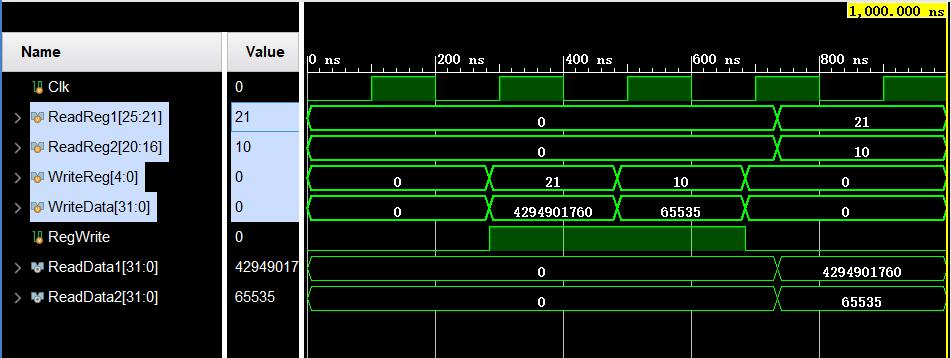
\includegraphics[width=0.9\textwidth]{fig-sim-reg.jpg}
    \caption{寄存器模块的仿真结果}
    \label{fig:sim-reg}
\end{figure}

\subsection{内存单元模块的仿真}
编写激励文件进行仿真,完整激励文件见dataMemory\_tb.v。仿真过程中,输入的测试信号如下:
\begin{lstlisting}[language=verilog]
//185ns
MemRead = 0;
MemWrite = 1;
Address = 32'b00000000000000000000000000000111;
WriteData = 32'b11100000000000000000000000000000;
#100;

//285ns
MemRead = 0;
MemWrite = 1;
WriteData = 32'hffffffff;
Address = 32'b00000000000000000000000000000110;
#185;

//470ns
MemRead = 1;
MemWrite = 0;
#80;

//550ns
MemRead = 1;
MemWrite = 1;
Address = 8;
WriteData = 32'haaaaaaaa;
#80;

//630ns
MemWrite = 0;
MemRead = 1;
\end{lstlisting}\par
仿真结果见图\ref{fig:sim-mem}。可以看出,内存读取结果readData出现两段x信号,其中,第一段是因为读取信号一直为低电平使得输出寄存器处于未初始化状态,待memRead信号第一次生效后便恢复正常;第二段是由于选取的内存地址本身没有被初始化,当时钟达到下降沿之后,数据被写入,输出也恢复了正常。由于本实验没有初始化要求,在与老师沟通交流后,我得知这样的结果也是正确的。
\begin{figure}[H]
    \centering
    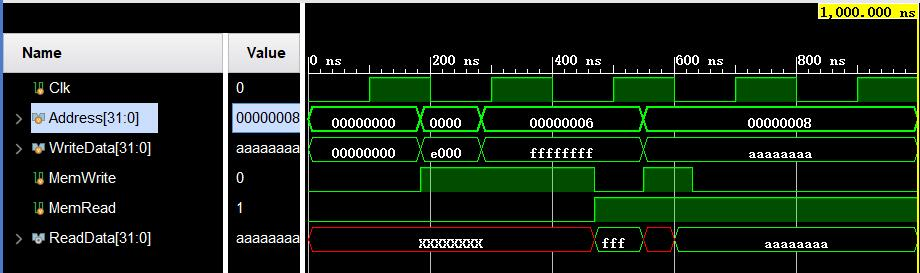
\includegraphics[width=0.9\textwidth]{fig-sim-mem.jpg}
    \caption{内存单元模块的仿真结果}
    \label{fig:sim-mem}
\end{figure}

\subsection{符号扩展模块的仿真}
编写激励文件进行仿真,完整激励文件见signext\_tb.v。仿真测试全程将signExt信号设置为高电平,使符号扩展模块运行在带符号扩展模式下,测试带符号扩展结果。激励文件会依次输入数据0、1、0xffff、2、0xfffe、0x8000、0x7f93。仿真结果如图\ref{fig:sim-ext}所示,符号扩展模块运行符合预期。
\begin{figure}[H]
    \centering
    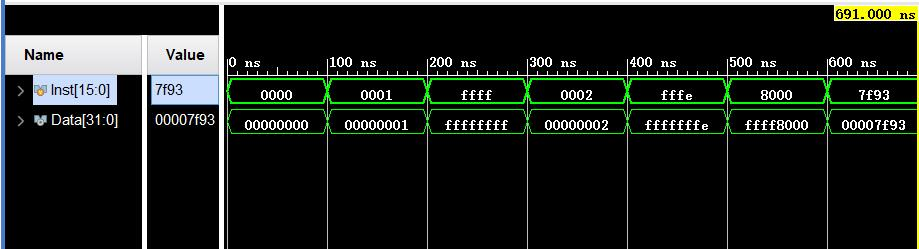
\includegraphics[width=0.9\textwidth]{fig-sim-ext.jpg}
    \caption{符号扩展模块的仿真结果}
    \label{fig:sim-ext}
\end{figure}
\section{总结与反思}\label{sec4}
在本实验中,我实现了寄存器模块、内存单元模块、符号扩展模块。本实验整体难度较低,但是通过完成本实验,我依然有较大收获。符号扩展模块的实现,让我熟悉了Verilog中的三目运算符与信号拼接操作。寄存器模块、内存单元模块让我学会了存储器的实现。\par
在内存单元模块的实现过程中,我遇到过当写入与读取同时进行时,读取输出信号无法及时同步的问题。在查阅资料并多次尝试后,我发现该问题是由于我用于暂存输出结果的寄存器没有及时更新数据造成的,通过将输出端口直接与对应寄存器相连,我顺利解决了这个问题。\par
结合实验4,我们实现了一个处理器的大部分功能模块。与计算机程序的实现思维类似,在硬件的设计过程中,也可以通过将功能细化,然后分别实现各模块,如此的实现思路,既便于团队开发,也便于后期维护。
\end{document}